\documentclass[conference]{IEEEtran}
\IEEEoverridecommandlockouts
% The preceding line is only needed to identify funding in the first footnote. If that is unneeded, please comment it out.
\usepackage{cite}
\usepackage{amsmath,amssymb,amsfonts}
\usepackage{algorithmic}
\usepackage{graphicx}
\usepackage{textcomp}
\usepackage{xcolor}
\usepackage{url}
\def\BibTeX{{\rm B\kern-.05em{\sc i\kern-.025em b}\kern-.08em
    T\kern-.1667em\lower.7ex\hbox{E}\kern-.125emX}}
\begin{document}

\title{Artificial Intelligence Agent for Pong using Deep Learning Techniques}
\author{
\IEEEauthorblockN{Brian Duke}
\IEEEauthorblockA{\textit{College of Computing and Informatics} \\
\textit{Drexel University}\\
Philadelphia, PA, USA}
\and 
\IEEEauthorblockN{Alan Harris}
\IEEEauthorblockA{\textit{College of Computing and Informatics} \\
\textit{Drexel University}\\
Philadelphia, PA, USA}
\and 
\IEEEauthorblockN{Shyam Desai}
\IEEEauthorblockA{\textit{College of Computing and Informatics} \\
\textit{Drexel University}\\
Philadelphia, PA, USA}
\and 
\IEEEauthorblockN{Umar Hassam}
\IEEEauthorblockA{\textit{College of Computing and Informatics} \\
\textit{Drexel University}\\
Philadelphia, PA, USA}
}

\maketitle

\begin{abstract}
Artificial intelligence (AI) agents for games are typically written with a set of rules and knowledge about their environment. With the recent availability of libraries that interface with game emulation, it is now possible to create an artificial intelligence (AI) agent that can learn to play the game. These methods, namely neuroevolution and reinforcement learning, are competitive alternatives to the traditional design of AI agents. In this paper, different models and learning techniques are compared for an AI that can play Pong. 
\end{abstract}

\begin{IEEEkeywords}
deep learning, genetic algorithm, reinforcement learning, artificial intelligence
\end{IEEEkeywords}

\section{Background}

\subsection{Pong}

Atari's game of Pong, released in 1972, is one of the first commercial video games. The rules of the game are simple. There are two players, either computer or human, that must use their paddle to hit a ball. The paddles can move up and down, or choose to do nothing. A player scores a goal when the ball goes behind the opponent's paddle at the end of the screen. The player with the most points at the end of the game wins. Pong's built-in computer player is an example of a traditional AI agent. The Pong computer player always moves its paddle to follow the Y position of the ball \cite{pong_info}.

The meaning of artificial intelligence is open to interpretation. While Pong's computer player falls under the category of AI, the argument could be made that is not a truly intelligent agent. A truly intelligent agent should be able to learn and compete in an environment without prior knowledge. Two methods that attempt to create intelligent agents are evolutionary algorithms and reinforcement learning. These methods tune weights in a neural network. The weights can be thought of as the dendrites and axons that are in a human brain. 

\subsection{Genetic algorithms}

Genetic Algorithm (GA) is a type of optimizing search. As the name implies, the GA is inspired by Darwin's theory of evolutionary biology. In GA, a population $Y$ of $n$ individuals (sometimes called genotypes or chromosomes) are initialized with random values. At every generation, each individual $n_i$ is evaluated by the fitness function. The fitness function's purpose is to maximize desirable traits. The next steps are selection, crossover, and mutation. In selection, a number of top individuals are selected to create the ``offspring" of the next generation. In crossover, the new offspring receives random traits from the parents pair. In mutation, there is a probability that an offspring's trait may change.

It can be seen how easily the idea of GA can be applied to deep learning. For a deep learning problem, the genotypes are the neural networks (specifically, the weights of the neural networks' fully connected layers). When a typical DNN converges for a problem with a high-dimensional problem space, it is doing so through gradient descent and backpropagation with ground truth data. For the design of an intelligent agent, the agent can not know previous results and their labeled outcomes. GA essentially replaces the backpropagation. The networks are still forward propagating through all of their layers. But now, the weights are tuned through GA \cite{DBLP:journals/corr/abs-1712-06567} \cite{katoch2021review}.

\subsection{Reinforcement learning}

Q-learning is a model-free method of reinforcement learning that works by mapping rewards to states, thus defining the value of a particular action for a state. The Bellman equation is at the core of this algorithm, defining the reward for actions taken at earlier points in time leading up to a final reward state. It uses a discount and learning rate factor, alongside the potential future reward from a given state and action to update this table repeatedly. The algorithm has proven to be remarkably successful at game AI problems in smaller state spaces. 

\begin{figure}[htbp]
    \centerline{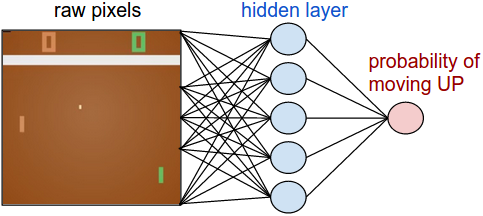
\includegraphics[width=0.4\textwidth]{policy.png}}
    \caption{Andrej Karpathy's Atari Policy RL Network}
    \label{andrejkarpathy}
\end{figure}

To expand this algorithm and incorporate a larger state space, the advent of Deep Reinforcement Learning has also shown much promise. In short, a neural network is used to map these state-to-action values. A particularly deep one has the ability to internalize a far greater number of states compared to a Q learning table. The policy network in Figure 1 demonstrates how this is possible with a relatively small architecture. A reasonable action can be learned from this architecture, and a reward state from the future can be used as a gradient (with past states getting diminished returns). Researchers have also stipulated that the inclusion of convolutional layers specifically for tasks relating to pixel level information such as Pong have shown promise.

\section{Related Work}

\begin{figure}[htbp]
\centerline{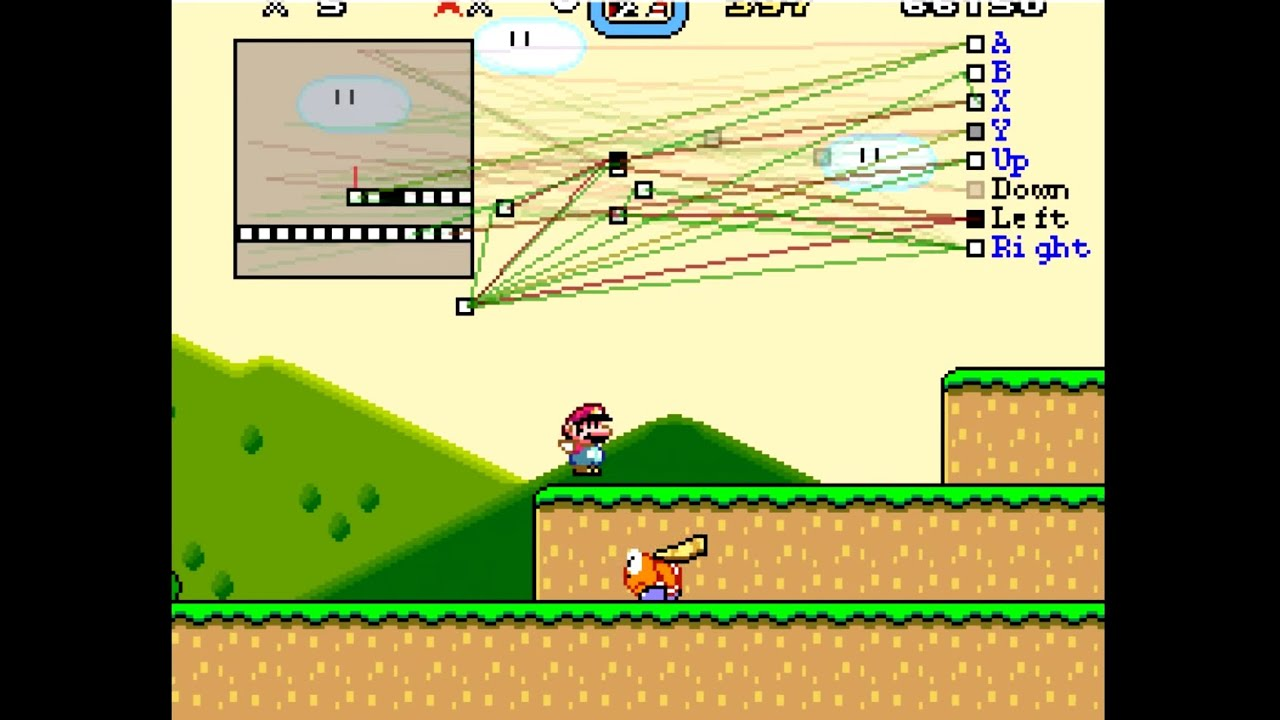
\includegraphics[width=0.4\textwidth]{sethbling.jpg}}
\caption{SethBling's MarI/O with a graphical representation of the network input, connections, and outputs.}
\label{sethbling}
\end{figure}

GA has been proven to be a competitive alternative to backpropagation. Such et al. used a Deep GA algorithm to train agents for Atari games. They speculated that GA can train a neural network better than/just as good as other methods because ``... sampling in the region around good solutions is often sufficient to find even better solutions" \cite{DBLP:journals/corr/abs-1712-06567}. 

The YouTube creator SethBling popularized GA for video game agents with his MarI/O project that plays Super Mario World \cite{mario}. MarI/O uses the NeuroEvolution of Augmenting Toplogies (NEAT) algorithm. This algorithm uses GA to evolve a neural network without assuming the best structure for the neurons' connections. It also separates genotypes into species \cite{stanley2002evolving}. Chris Presso trained a neural net with GA to play Super Mario Bros \cite{presso}. 

\section{Methodology}

\begin{figure}[htbp]
\centerline{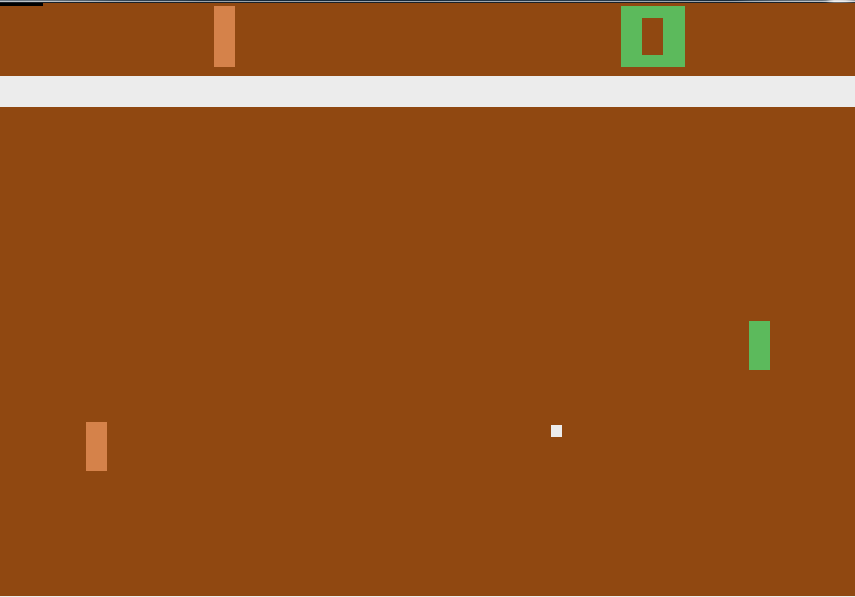
\includegraphics[width=0.35\textwidth]{pong2600.png}}
\caption{Pong for the Atari 2600 running in Gym.}
\label{pong2600}
\end{figure}

This section discusses the architecture, hyperparameters, libraries, and algorithms in designing Pong agents. 

\subsection{Libraries}

OpenAI's Gym is a Python library that allows for the development and training of video game AI agents \cite{DBLP:journals/corr/BrockmanCPSSTZ16}. Gym can load environments for retro and classic video games. The environment is the state information about a game, retrieved as either pixels or RAM data. The Arcade Learning Environment (ALE) is an expansion for Gym \cite{DBLP:journals/corr/abs-1709-06009}. ALE gives a collection of ROMs for the Atari 2600 and their respective environment information. We used ALE to load the Pong ROM for Atari 2600. For our CS615 Deep Learning class, we did not use any learning libraries. The neural nets, genetic algorithm, and other parts of the learning were implemented from scratch. The NumPy library was used.

\subsection{Algorithms}

The Python script begins by initializing the parameters. For the simple game of Pong, we decided that a population of 20 individuals should be trained for 40 generations. Each generation of training takes about thirty seconds. In each generation, each individual plays a game of pong against the Pong computer agent. 

\begin{equation}\label{arch}
\text{Input} \rightarrow \text{Full (2640)} \rightarrow \text{Softmax} \rightarrow \text{GA}
\end{equation}

To be clear, there is not an actual input layer. The input is pre-processed with the library Pillow. The game pixels are converted to grayscale, cropped, and scaled to a 60x44 size image.

The current input image is subtracted from the previous to provide velocity information. Each game only last for a maximum of 1000 frames before ending.

The fitness function was tuned to reward movement over no movement, reward gaining score over the opponent, and too discourage allowing the opponent to score by subtracting fitness.

\begin{enumerate}
\item test1
\item test2
\end{enumerate}


\section{Experiments and Results}

\begin{figure}[htbp]
\centerline{\includegraphics[width=0.4\textwidth]{GNN_figure.png}}
\caption{The training plataeu shows overfitting.}
\label{overfitting}
\end{figure}

\begin{figure}[htbp]
\centerline{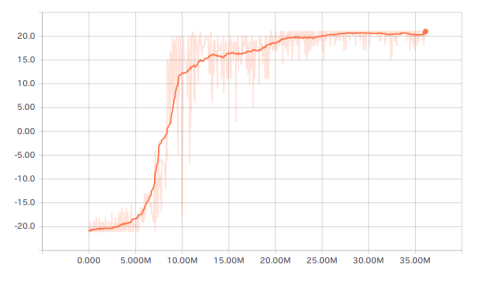
\includegraphics[width=0.4\textwidth]{rl__graph.png}}
\caption{Average Pong Score over simulation (millions) for Makarov et al. Deep Reinforcement Learning Implementation}
\label{overfitting}
\end{figure}



\section{Conclusions}

To conclude, we found that the GA approach to learning can produce good results in circumstances where training data in not labeled. This approach inspired by genetic evolution performs best with a large enough population size and enough generations.

Though our example showed overfitting, obeserving the trained AI play showed that it evolved from random inputs to something resembling a strategy but only for one section of the game window as the training data did not vary enough between runs to adjust for other sections.

With a larger population size, more generations, and with a more stochastic version of Pong, the trained AI could perform well enough to compete with the pre-coded traditional Pong AI.

\section{Future Work}

To avoid the pit-falls of overfitting that was observed during training with the GA, changing the version of Pong can yield better results. There is a need for ball stochasticity as there is no good way to get ball stochasticity in the Atari ROM.

Changing the fitness function after some convergence could also be used to encourage certain behaviors and avoid local minimum. This could be used to discourage unneeded movement in pong after it has begun to score points.

\bibliography{mybib}{}
\bibliographystyle{plain}

\vspace{12pt}

\end{document}
